\documentclass[12pt,]{article}
\usepackage{lmodern}
\usepackage{amssymb,amsmath}
\usepackage{ifxetex,ifluatex}
\usepackage{fixltx2e} % provides \textsubscript
\ifnum 0\ifxetex 1\fi\ifluatex 1\fi=0 % if pdftex
  \usepackage[T1]{fontenc}
  \usepackage[utf8]{inputenc}
\else % if luatex or xelatex
  \ifxetex
    \usepackage{mathspec}
    \usepackage{xltxtra,xunicode}
  \else
    \usepackage{fontspec}
  \fi
  \defaultfontfeatures{Mapping=tex-text,Scale=MatchLowercase}
  \newcommand{\euro}{€}
\fi
% use upquote if available, for straight quotes in verbatim environments
\IfFileExists{upquote.sty}{\usepackage{upquote}}{}
% use microtype if available
\IfFileExists{microtype.sty}{%
\usepackage{microtype}
\UseMicrotypeSet[protrusion]{basicmath} % disable protrusion for tt fonts
}{}
\usepackage[margin=1in]{geometry}
\usepackage{graphicx}
\makeatletter
\def\maxwidth{\ifdim\Gin@nat@width>\linewidth\linewidth\else\Gin@nat@width\fi}
\def\maxheight{\ifdim\Gin@nat@height>\textheight\textheight\else\Gin@nat@height\fi}
\makeatother
% Scale images if necessary, so that they will not overflow the page
% margins by default, and it is still possible to overwrite the defaults
% using explicit options in \includegraphics[width, height, ...]{}
\setkeys{Gin}{width=\maxwidth,height=\maxheight,keepaspectratio}
\ifxetex
  \usepackage[setpagesize=false, % page size defined by xetex
              unicode=false, % unicode breaks when used with xetex
              xetex]{hyperref}
\else
  \usepackage[unicode=true]{hyperref}
\fi
\hypersetup{breaklinks=true,
            bookmarks=true,
            pdfauthor={},
            pdftitle={},
            colorlinks=true,
            citecolor=blue,
            urlcolor=black,
            linkcolor=black,
            pdfborder={0 0 0}}
\urlstyle{same}  % don't use monospace font for urls
\setlength{\parindent}{0pt}
\setlength{\parskip}{6pt plus 2pt minus 1pt}
\setlength{\emergencystretch}{3em}  % prevent overfull lines
\setcounter{secnumdepth}{0}

%%% Use protect on footnotes to avoid problems with footnotes in titles
\let\rmarkdownfootnote\footnote%
\def\footnote{\protect\rmarkdownfootnote}

%%% Change title format to be more compact
\usepackage{titling}

% Create subtitle command for use in maketitle
\newcommand{\subtitle}[1]{
  \posttitle{
    \begin{center}\large#1\end{center}
    }
}

\setlength{\droptitle}{-2em}
  \title{}
  \pretitle{\vspace{\droptitle}}
  \posttitle{}
  \author{}
  \preauthor{}\postauthor{}
  \date{}
  \predate{}\postdate{}

\usepackage{lineno}
\linenumbers
\usepackage{setspace}
\usepackage{todonotes}
\doublespacing
\usepackage{rotating}
\usepackage{color, soul}
\usepackage[font={footnotesize},labelfont={sf,bf},labelsep=space]{caption}
\usepackage{sectsty}

\begin{document}

\maketitle


\renewcommand\linenumberfont{\normalfont\tiny\sffamily\color{gray}}

\newcommand{\tc}{\textcolor}

\begin{singlespace}

\begin{centering}

\Large{The relationship between species richness and ecosystem variability is shaped by the mechanism of coexistence}

\vspace{2.5em}

\renewcommand*{\thefootnote}{\fnsymbol{footnote}}

\normalsize{Andrew T. Tredennick\textsuperscript{1}, Peter B. Adler\textsuperscript{1}, and Frederick R. Adler\textsuperscript{2}}

\vspace{1.5em}

\textit{\small{\textsuperscript{1}Department of Wildland Resources and the Ecology Center, Utah State University, Logan, Utah 84322}} \\
\textit{\small{\textsuperscript{2}Departments of Biology and Mathematics, University of Utah, Salt Lake City, Utah 84112}} 

\end{centering}

\vspace{3em}

Last compile: \today

\noindent \textbf{Keywords}: coexistence, storage effect, relative nonlinearity, diversity-stability hypothesis, pulsed differential equation, consumer-resource dynamics

\noindent \textbf{Authorship}: All authors conceived the research and designed the modeling approach; ATT conducted model simulations, with input from PBA and FRA; ATT wrote the manuscript and all authors contributed to revisions.

\noindent \textbf{Data Accessibility}: There is no data associated with this manuscript. All R code necessary to reproduce our results will be archived on Figshare and released on GitHub (https://github.com/atredennick/Coexistence-Stability).

\noindent \textbf{Running Title}: Environmental variability, ecosystem variability, \& species coexistence

\noindent \textbf{Article Type}: Letter

\noindent \textbf{Number of Words}: 3,699

\noindent \textbf{Number of Words in Abstract}: 147

\noindent \textbf{Number of References}: 40

\noindent \textbf{Number of Tables and Figures}: 1 table, 5 figures

\noindent \textbf{Corresponding Author}:  \\
\phantom{222}Andrew Tredennick  \\
\phantom{222}Department of Wildland Resources and the Ecology Center  \\
\phantom{222}Utah State University  \\
\phantom{222}5230 Old Main Hill  \\
\phantom{222}Logan, Utah 84322 USA  \\
\phantom{222}Phone: +1-970-443-1599  \\
\phantom{222}Fax: +1-435-797-3796  \\
\phantom{222}Email: atredenn@gmail.com

\end{singlespace}

\newpage{}

\begin{abstract}
Theory relating species richness to ecosystem variability typically ignores the potential for environmental variability to promote species coexistence.
Failure to account for fluctuation-dependent coexistence mechanisms may explain observed deviations from the expected negative diversity-variability relationship, and limits our ability to predict the consequences of future increases in environmental variability.
We use a consumer-resource model to explore how coexistence via the temporal storage effect and relative nonlinearity affects ecosystem variability.
We show that a positive, rather than negative, diversity-variability relationship is possible when ecosystem function is sampled across a natural gradient in environmental variability and diversity.
We also show how fluctuation-dependent coexistence can buffer ecosystem functioning against increasing environmental variability by promoting species richness and portfolio effects.
Our work provides a general explanation for variation in observed diversity-variability relationships and highlights the importance of conserving regional species pools to help buffer ecosystems against predicted increases in environmental variability.
\vspace{2em}
\end{abstract}

\newpage{}

\setlength{\parindent}{5ex}

\subsection{INTRODUCTION}\label{introduction}

MacArthur (1955), Elton (1958), and even Darwin (Turnbull et al. 2013)
recognized the potential for compensatory dynamics among species to
stabilize ecosystem functioning in fluctuating environments. This idea
underlies the ``insurance hypothesis'' (Yachi \& Loreau 1999), which
suggests ecosystem variability decreases with diversity because species
respond dissimilarly to environmental variation, broadening the range of
conditions under which the community maintains function (Loreau 2010). A
variety of theoretical models all predict a negative relationship
between species richness and ecosystem variability (Lehman \& Tilman
2000; Ives \& Hughes 2002; Loreau \& {{de Mazancourt}} 2013), and
experimental tests tend to support such a prediction (Tilman et al.
2006; Hector et al. 2010).

However, the ability of biodiversity-ecosystem functioning (BEF)
experiments to accurately represent real-world dynamics is debated
(Eisenhauer et al. 2016; Wardle 2016). Much of the debate centers on the
fact that BEF experimental protocols do not allow species gains to
offset species losses. Theoretical work on diversity-variability
relationships typically suffers from the same limitation: it recognizes
the role of environmental variability in driving population fluctuations
which destabilize ecosystems, but ignores the potential for
environmental variability to promote species richness and thereby help
stabilize ecosystems (Loreau 2010, but see Chesson et al. 2001).

Fluctuating environmental conditions are an important ingredient for
stable species coexistence, both in theoretical models (Chesson 2000a;
Chesson et al. 2004) and in natural communities (C{á}ceres 1997;
Descamps-Julien \& Gonzalez 2005; Adler et al. 2006; Angert et al.
2009). Such ``fluctuation-dependent'' coexistence requires that species
have unique environmental responses and that environmental conditions
vary so that each species in a community experiences favorable and
unfavorable conditions, which prevents competitive exclusion (Chesson
2000a). When coexistence is maintained by a fluctuation-dependent
mechanism, an increase in environmental variability might lead to an
increase in species richness and, consequently, a decrease in ecosystem
variability. However, increasing environmental variability may also
increase ecosystem variability by increasing the fluctuations of
individual species, regardless of species richness. These countervailing
effects of environmental variability present an interesting paradox:
while we should expect an increase in environmental fluctuations to
increase ecosystem variability, this increase might be buffered if
fluctuation-dependent coexistence adds new species to the community.
Such a paradox complicates predictions about how ecosystems will respond
to predicted departures from historical ranges of environmental
variability.

The opposing effects of environmental variability on ecosystem
variability might explain the mixed results from empirical studies on
the diversity-variability relationship. Observational tests of the
diversity-variability relationship, which require sampling across
natural diversity gradients, have yielded negative (Hautier et al.
2014), neutral (Valone \& Hoffman 2003; Cusson et al. 2015), and
positive (Sasaki \& Lauenroth 2011) relationships. In a meta-analysis of
diversity-variability relationships based on observational studies in
terrestrial ecosystems, Jiang \& Pu (2009) found no significant evidence
for an effect of species richness on ecosystem variability, perhaps
because environmental variability varies across natural diversity
gradients, affecting both richness and ecosystem variability. The
idiosyncratic results of these empirical studies contrast with the
consistent conclusions from theoretical work that ignores feedbacks
between variability and richness.

The gap between theoretical expectations and empirical results of
richness-variability relationships might reflect the divergence of
theory developed to explain species coexistence and theory developed to
explain diversity and ecosystem variability. One reason these two
disciplines have diverged is because they have focused on different
questions. Diversity-variability studies typically ask how ecosystem
variability responds to different levels of species richness at a given
level of environmental variability (reviewed in Kinzig et al. 2001;
Loreau 2010), whereas coexistence studies ask how species richness
responds to different levels of environmental variability (Chesson \&
Warner 1981).

To reconcile these two perspectives, we extend theory on the
relationship between species richness and ecosystem variability to cases
in which species coexistence explicitly depends on environmental
fluctuations and species-specific responses to environmental conditions.
We focus on the temporal storage effect and relative nonlinearity using
a general consumer-resource model. We use the model to investigate two
questions:

\begin{enumerate}
\def\labelenumi{\arabic{enumi}.}
\item
  Does the diversity-variability relationship remain negative when
  species coexistence is maintained by the temporal storage effect or
  relative nonlinearity?
\item
  How does increasing environmental variability impact ecosystem
  variability when coexistence depends on the storage effect or relative
  nonlinearity?
\end{enumerate}

\subsection{MATERIALS AND METHODS}\label{materials-and-methods}

\subsubsection{Consumer-resource model}\label{consumer-resource-model}

We developed a semi-discrete consumer-resource model that allows many
species to coexist on one resource by either the storage effect or
relative nonlinearity. In our model, the consumer can be in one of
two-states: a dormant state \(D\) and a live state \(N\). The dormant
state could represent, for example, the seed bank of an annual plant.
Transitions between \(N\) and \(D\) occur at discrete intervals \(\tau\)
with continuous-time consumer-resource dynamics between discrete
transitions. Thus, our model is formulated as ``pulsed differential
equations'' (Pachepsky et al. 2008; Mailleret \& Lemesle 2009; Mordecai
et al. 2016). For clarity we refer to \(\tau\) as years and the growing
time between years as seasons with daily (\(t\)) time steps.

During a growing season, consumer-resource dynamics are modeled as two
differential equations: \vspace{-3em}

\begin{align}
\frac{\text{d}N_{i}}{\text{d}t} &= \epsilon_if_{i}(R)N_{i}, \quad t \ne \tau_k\\
\frac{\text{d}R}{\text{d}t} &= - \sum\limits_{i}f_{i}(R)N_{i}, \quad t \ne \tau_k
\end{align}\vspace{-3em}

\noindent where the discrete transitions between \(N\) and \(D\) occur
between seasons at times \(\tau_k\), \(k = 1,2,3, \dots, K\). The
subscript \(i\) denotes species, \(N\) is the living biomass state, and
\(\epsilon_i\) is each species' resource-to-biomass conversion
efficiency. The growth rate of living biomass is a resource-dependent
Hill function,
\(f_{i}(R) = r_{i}R^{a_{i}} / (b_{i}^{a_{i}}+R^{a_{i}})\), where
\emph{r} is a species' intrinsic growth rate and \emph{a} and \emph{b}
define the curvature of the function. Resource depletion is equal to the
sum of each species' consumption.

Along with resource uptake, consumer population growth depends on the
production of dormant biomass (\(D\)), the activation of dormant biomass
to live biomass (\(D \rightarrow N\)), and the survival of living
biomass from one year to the next. The biomass of each species' states
at the start of a growing season are equal to \vspace{-3em}

\begin{align}
  D_{i}(\tau_k^+) &= (1-\gamma_{i,\tau_k})[\alpha_i N_{i}(\tau_k) + D_{i}(\tau_k)](1-\eta_i) \\
  N_{i}(\tau_k^+) &= (1-\alpha_i)N_{i}(\tau_k) + \gamma_{i,t}[\alpha_i N_{i}(\tau_k) + D_{i}(\tau_k)] (1-\eta_i),
\end{align}\vspace{-3em}

\noindent where \(D(\tau_k)\), \(N(\tau_k)\), and \(R(\tau_k)\) are the
abundances of each state at the end of growing season \emph{k} and
\(\tau_k^+\) denotes the beginning of growing season \(k+1\). The
activation of dormant biomass to live biomass is controlled by
\(\gamma\), which is year (\emph{k}) and species (\emph{i}) specific.
Dormant biomass is equal to a constant fraction (\(\alpha\)) of live
biomass at the end of the previous season (\(N_{i}(\tau_k)\)), plus
survival (\(1-\eta_i\)) of dormant biomass (\(D_{i}(\tau_k)\)) at the
end of the previous year and dormant biomass remaining after live
biomass activation (\(D_{i}(\tau_k)(1-\gamma_{i,\tau_k})\)). Live
biomass is equal to newly activated dormant biomass
(\(\gamma_{i,t}D_{i}(\tau_k)\)), minus some fraction of live biomass
that is converted to dormant biomass (\((1-\alpha_i)N_{i}(\tau_k)\)) We
assume the resource pool is not replenished within a growing season.
Resource replenishment occurs between growing seasons, and the resource
pool (\emph{R}) at the start of the growing season \emph{k}+1 is
\(R(\tau_k^+) = R^+\), where \(R^+\) is a random resource pulse drawn
from a log-normal distribution with mean \(\mu(R^+)\) and standard
deviation \(\sigma(R^+)\). Model parameters and notation are described
in Table 1.

\paragraph{Implementing the Storage
Effect}\label{implementing-the-storage-effect}

For the storage effect to operate, we need species-specific responses to
environmental variability, density-dependent covariance between
environmental conditions and competition (\emph{EC} covariance), and
subadditive population growth (Chesson 1994, 2000b). Long-term
coexistence is possible when all species can increase when rare. In the
storage effect, rare species increase by escaping the effects of
\emph{EC} covariance. Common species will experience greater than
average competition (\emph{C}) in good environment (\emph{E}) years
because common species cannot avoid intraspecific competition. However,
rare species can escape intraspecific competition and have the potential
to increase rapidly in a good \emph{E} year. \emph{EC} covariance
emerges in our model because dormant-to-live transition rates
(\(\gamma\)) are species-specific and vary through time. In a high
\(\gamma\) year for a common species, resource uptake will be above
average, while in a high \(\gamma\) year for a rare species, resource
uptake will be below average, as long as \(\gamma\)s are not perfectly
correlated between species. Subadditive population growth buffers
populations against large population decreases in unfavorable years. It
is included in our model through a dormant stage with very low death
rates, which limits large population declines in bad \emph{E} years.

We generated sequences of (un)correlated dormant-to-live state
transition rates (\(\gamma\)) for each species by drawing from
multivariate normal distributions with mean 0 and a variance-covariance
matrix (\(\Sigma(\gamma)\)) of \vspace{-3em}

\begin{align}
\Sigma(\gamma) = 
\begin{bmatrix}
1 & \rho_{1,2} & \rho_{1,3} & \rho_{1,4} \\
\rho_{2,1} & 1 & \rho_{2,3} & \rho_{2,4} \\
\rho_{3,1} & \rho_{3,2} & 1  & \rho_{3,4} \\
\rho_{4,1} & \rho_{4,2} & \rho_{4,3} & 1  \\
\end{bmatrix}
\sigma_{E}^2,
\end{align}\vspace{-2em}

\noindent where \(\sigma^2_{E}\) is the variance of the environmental
cue and \(\rho_{i,j}\) is the correlation between species \emph{i}'s and
species \emph{j}'s transition rates. \(\rho\) must be less than 1 for
stable coexistence, and in all simulations we constrained all
\(\rho_{i,j}\)'s to be equal. In a two-species community, the inferior
competitor has the greatest potential to persist when \(\rho=-1\)
(perfectly uncorrelated transition rates). However, in a four-species
community the minimum possible correlation among species is -1/3 given
our constraints that all \(\rho\)'s are equal and that
\(\Sigma(\gamma)\) must be positive-definite. We used the \texttt{R}
function \texttt{mvrnorm} to generate sequences of (un)correlated
variates \emph{E} that we converted to germination rates in the 0-1
range: \(\gamma = e^E / \left(1 + e^E \right)\).

\paragraph{Implementing Relative
Nonlinearity}\label{implementing-relative-nonlinearity}

In the absence of environmental fluctuations, the outcome of competition
between two species limited by the same resource is determined by the
shape of their resource uptake curves. That is, at constant resource
supply, whichever species has the lowest resource requirement at
equilibrium (\(R^*\)) will exclude all other species (Tilman 1982).
Resource fluctuations create opportunities for species coexistence
because the resource level will sometimes exceed the \(R^*\) of the
superior competitor. If the resource uptake curves of each species are
relatively nonlinear, then some species will be able to take advantage
of resource levels that other species cannot (Chesson 1994).

For example, in Fig. 1C we show uptake curves of two species with
different degrees of nonlinearity. Species B has the lowest \(R^*\) and
would competitively exclude species A in the absence of environmental
fluctuations. But fluctuating resource supplies can benefit species A
because it can take advantage of relatively high resource levels due its
higher saturation point. Stable coexistence is only possible, however,
if when each species is dominant it improves conditions for its
competitor. This occurs in our model because when a resource
conservative species (e.g., species B in Fig. 1C) is abundant, it will
draw resources down slowly after a pulse, and its competitor can take
advantage of that period of high resource availability. Likewise, when a
resource acquisitive species (e.g., species A in Fig. 1C) is abundant,
after a pulse it quickly draws down resources to levels that favor
resource conservative species. Such reciprocity helps each species to
increase when rare, stabilizing coexistence (Armstrong \& McGehee 1980;
Chesson 2000a; Chesson et al. 2004).

\subsubsection{Numerical simulations}\label{numerical-simulations}

To explore how fluctuation-dependent coexistence can affect the
diversity-variability relationship, we simulated the model with four
species under two scenarios for each coexistence mechanism. First, we
allowed the variance of the environment to determine how many species
can coexist, akin to a community assembly experiment with a species pool
of four species. To do this, we simulated communities with all species
initially present across a gradient of annual resource variability (for
relative nonlinearity) or environmental cue variability (for the storage
effect). Second, we chose parameter values that allowed coexistence of
all four species and then performed species removals, akin to a
biodiversity-ecosystem function experiment. The two simulation
experiments correspond to (i) sampling ecosystem function across a
natural gradient of species richness and (ii) sampling ecosystem
function across diversity treatments within a site.

To understand how increasing environmental variability will impact
ecosystem variability when coexistence is fluctuation-dependent, we
simulated the model over a range of species pool sizes and environmental
cue or resource variability. For each size of species pool (1, 2, 3, or
4 species), we simulated the model at 15 evenly-spaced levels of
environmental cue (range = 0.1,2) for the storage effect and 25
evenly-spaced levels of resource variability (range = 0.1,1.4) for
relative nonlinearity. We also explored the influence of asymmetries in
species' competitive abilities and correlations in species'
environmental responses within the storage effect model.

Under relative nonlinearity, species' resource response curves (Fig.
S1-1) reflect traits that determine the temporal variability of each
species' population growth. ``Stable'' species achieve maximum resource
uptake at low resource levels, but their maximum uptake rates are
modest. For these species, population responses to resource fluctuations
are buffered. ``Unstable'' species have very high maximum uptake rates,
which they only achieve when resource availability is high, leading to
large population fluctuations. The difference in the intrinsic stability
of these two kinds of species makes our simulations sensitive to initial
conditions. Therefore, we ran two sets of simulations for relative
nonlinearity: beginning with either stable or unstable species as a
reference point For example, if species A is the most stable species and
species D is the least stable, we ran simulations where A then B then C
then D were allowed to invade. We then ran simulations with that order
reversed.

All simulations were run for 5,000 growing seasons of 100 days each. We
averaged biomass over the growing season, and those yearly values were
used to calculate total community biomass in each year. After discarding
an initial 500 seasons to reduce transient effects on our results, we
calculated the coefficient of variation (\emph{CV}) of summed species
biomass through time, which represents ecosystem variability, the
inverse of ecosystem stability. We calculated species richness as the
number of species whose average biomass was greater than 1 over the
course of the simulation. Parameter values for specific results are
given in figure captions. Within-season dynamics were solved given
initial conditions using the package \texttt{deSolve} (Soetaert et al.
2010) in \texttt{R} (Team 2013). \texttt{R} code for our model function
is in the Supporting Information Appendix S1. All model code has been
deposited on Figshare (\emph{link}) and is available on GitHub at
\url{http://github.com/atredennick/Coexistence-Stability}.

\subsection{RESULTS}\label{results}

When we allowed the variance of the environment to determine which of
four initial species coexisted, similar to a study across a natural
diversity gradient, we found a positive relationship between richness
and variability (Fig. 2A,C). This was true for the storage effect, where
coexistence is maintained by fluctuating dormant-to-live transition
rates (\(\gamma\)), and for relative nonlinearity, where coexistence is
maintained by annual resource pulses. The relationship is driven by the
fact that increasing environmental variability increases the strength of
both coexistence mechanisms (Fig. S1-2). More variable conditions
promoted species richness, creating a positive relationship between
diversity and variability.

When we performed species removals but held environmental variability at
a level that allows coexistence of all four species, similar to a
biodiversity-ecosystem functioning experiment, we found a negative
diversity-variability relationship (Fig. 2B,D). Scatter around the
relationship was small for the storage effect because all species have
similar temporal variances. Regardless of species identity, the presence
of more species always stabilized ecosystem functioning through
portfolio effects. In contrast, scatter around the relationship was
larger for relative nonlinearity (Fig. 2D) because species with
different resource uptake curves had different population variances.
Depending on which species were present, two-species communities were
sometimes less variable than three-species communities.

To understand how much species additions can stabilize ecosystem
functioning as environmental variability increases, we simulated our
model over a range of environmental variance and species pool sizes.
Realized species richness increased with environmental variability and,
in some cases, increases in richness completely offset the effect of
increasing environmental variability on ecosystem variability. More
species rich communities were less variable on average and increased in
ecosystem \emph{CV} at a slower rate than communities with fewer species
(e.g., lower slopes in log-log space; Fig. S1-3).

The dampening effect of fluctuation-dependent coexistence on increasing
environmental variability depends on the specific traits (parameter
values) of the species in the regional pool. Moderate competition makes
it more difficult for new species to enter the local community, but once
they do enter, variability is similar between communities with low and
moderate competition (Fig. 3; compare top and bottom panels). Moderate
competition does increase the rate at which ecosystem \emph{CV}
increases with environmental variance (Fig. S1-3) because the abundance
of inferior competitors is reduced and they do not influence ecosystem
\emph{CV} as much as when competition is low. The correlation of
species' environmental responses also mediates the relationship between
environmental variance, species richness, and ecosystem \emph{CV}: lower
correlations make it easier for new species to enter the community and
contribute to porfolio effects (Fig. 3).

In communities where species coexist via relative nonlinearity, the
extent to which species additions buffer ecosystem stability against
increases in environmental variability depends on the species traits of
immigrating species and the order in which they enter the community.
When additional species, which immigrate from the regional pool, are
less intrinsically stable than the resident species, ecosystem
variability increases at a constant rate even as species are added (Fig.
4A). If more stable species colonize, species additions buffer the
ecosystem from increasing environmental variability (Fig. 4B). When only
the most unstable (resource acquisitive) species is present, ecosystem
variability initially declines as resource variability increases (Fig.
4B) because for this species' monoculture biomass is very low at low
average resource levels for this species, inflating the \emph{CV}.

\subsection{DISCUSSION}\label{discussion}

Theory developed for biodiversity-ecosystem function experiments
emphasizes that increases in species richness should reduce ecosystem
variability. Consistent with theoretical expectations from models and
with results from biodiversity-ecosystem functioning experiments, in
which species coexistence is maintained by fluctuation-independent
mechanisms, our model of fluctuation-dependent species coexistence (also
see Chesson et al. 2001) produced a negative diversity-variability
relationship (Fig. 2B,D). This agreement is encouraging because species
almost certainly coexist by some combination of fluctuation-independent
(e.g., resource partitioning) and fluctuation-dependent mechanisms. By
extending theory to communities where species richness is explicitly
maintained by temporal variability, we have gained confidence that
experimental findings are generalizable to many communities. In local
settings where environmental variability is relatively homogeneous,
reductions in the number of species should increase the variability of
ecosystem functioning, regardless of how coexistence is maintained.

When we allowed communities to assemble at sites across a gradient of
environmental variability, we discovered a positive relationship between
species richness and ecosystem variability (Fig. 2A,C). While surprising
when viewed through the lens of biodiversity-ecosystem functioning
theory and experimental findings, such a relationship is predicted by
theory on coexistence in fluctuating environments. Environmental
variability is a prerequisite for the storage effect and relative
nonlinearity to stabilize coexistence (Chesson 2000a). These mechanisms
can translate increased variability into higher species richness (Fig.
S1-2), but the increase in environmental variability also increases
ecosystem variability.

Our results may explain why deviations from the negative
diversity-variability relationship often come from observational studies
(Jiang \& Pu 2009). Observational studies must rely on natural diversity
gradients, which do not control for differences in environmental
variability among sites. If species richness depends on environmental
variability, it is entirely possible to observe positive
diversity-variability relationships. For example, Sasaki and Lauenroth
(2011) found a positive relationship between species richness and the
temporal variability of plant abundance in a semi-arid grassland. Their
data came from a six sites that were 6 km apart. While Sasaki and
Lauenroth explained their results in terms of dominant species' effects,
it is also possible that each site experienced sufficiently different
levels of environmental variability to influence species coexistence.
DeClerck et al. (2006) also found a positive diversity-variability when
sampling conifer richness and the variability of productivity across a
large spatial gradient in the Sierra Nevada.

While our modeling results show that fluctuation-dependent coexistence
can create positive diversity-variability relationships, whether such
trends are detected will depend on the particular traits of the species
in the community and the relative influence of fluctuation-dependent and
fluctuation-independent coexistence mechanisms. Thus, our results may
also help explain observational studies where no relationship between
diversity and variability is detected. For example, Cusson et al. (2015)
found no relationship between species richness and variability of
abundances in several marine macro-benthic ecosystems. Many of their
focal ecosystems were from highly variable intertidal environments. If
coexistence was at least in part determined by environmental
fluctuations, then the confounding effect of variability and species
richness could offset or overwhlem any effect of species richness on
variability. Previous theoretical work showed how environmental
variation can mask the effect of species diversity on ecosystem
productivity when sampling across sites (Loreau 1998). Our mechanistic
model extends that conclusion to ecosystem variability.

Whether coexistence is fluctuation-independent or fluctuation-dependent
becomes especially important when we consider how ecosystem variability
responds to increasing environmental variability. In the
fluctuation-independent case, species richness is essentially fixed
because the niche and fitness differences that determine coexistence are
not linked to environmental variability. Therefore, increasing
environmental variability will always increase ecosystem variability by
increasing the fluctuations of individual species' abundances. When
coexistence is fluctuation-dependent, however, the outcome is less
certain. By simulating communities with different species pool sizes
across a gradient of environmental variability, we showed that species
gains due to increasing environmental variability can buffer the direct
effect of environmental variability on ecosystem variability (Figs. 3
and 4). These results lead to two conclusions.

First, when predicting the impacts of increasing environmental
variability on ecosystem variability, the mechanism of coexistence
matters. Fluctuation-dependent coexistence can buffer ecosystems from
increasing environmental variability by promoting increased species
richness. Whether our theoretical predictions hold in real communities
is unknown and requires empirical tests. Doing so would require
manipulating environmental variability in communities where coexistence
is known to be fluctuation-dependent, at least in part. Such data do
exist (Angert et al. 2009), and a coupled modeling-experimental approach
could determine if our predictions hold true in natural communities.

Second, whether local fluctuation-dependent communities can receive the
benefit of additional species depends on a diverse regional species
pool. If the regional pool is not greater in size than the local species
pool, than ecosystem variability will increase with environmental
variability in a similar manner as in fluctuation-independent
communities because species richness will be fixed (Fig. 5A,B).
Metacommunity theory has made clear the importance of rescue effects to
avoid species extinctions (Brown \& Kodric-Brown 1997; Leibold et al.
2004). Here, instead of local immigration by a resident species working
to rescue a species from extinction, immigration to the local community
by a new species rescues ecosystem processes from becoming more variable
(Fig. 5C,D). Thus, our results reinforce the importance of both local
and regional biodiversity conservation. Just as declines in local
species richness can destabilize ecosystem functioning (Tilman et al.
2006; Hector et al. 2010; Hautier et al. 2014), species losses at larger
spatial scales can also increase ecosystem variability. Wang \& Loreau
(2014) show that regional ecosystem variability depends on regional
biodiversity through its effects on beta diversity and, in turn, the
asynchrony of functioning in local communities. Our results show that,
when coexistence is fluctuation-dependent, regional biodiversity
declines could also affect local ecosystem functioning by limiting local
colonization events that could be possible under scenarios of increasing
environmental variability (Fig. 5).

\subsection{ACKNOWLEDGMENTS}\label{acknowledgments}

The National Science Foundation provided funding for this work through a
Postdoctoral Research Fellowship in Biology to ATT (DBI-1400370) and a
CAREER award to PBA (DEB-1054040).

\newpage{}

\setlength{\parindent}{0ex} \singlespacing

\subsection*{REFERENCES}\label{references}
\addcontentsline{toc}{subsection}{REFERENCES}

Adler, P.B., HilleRisLambers, J., Kyriakidis, P.C., Guan, Q. \& Levine,
J.M. (2006). Climate variability has a stabilizing effect on the
coexistence of prairie grasses. \emph{Proceedings of the National
Academy of Sciences}, 103, 12793--12798.

Angert, A.L., Huxman, T.E., Chesson, P. \& Venable, D.L. (2009).
Functional tradeoffs determine species coexistence via the storage
effect. \emph{Proceedings of the National Academy of Sciences of the
United States of America}, 106, 11641--11645.

Armstrong, R.A. \& McGehee, R. (1980). Competitive Exclusion. \emph{The
American Naturalist}, 115, 151--170.

Brown, J.H. \& Kodric-Brown, A. (1997). Turnover Rates in Insular
Biogeography : Effect of Immigration on Extinction. \emph{Ecology}, 58,
445--449.

C{á}ceres, C.E. (1997). Temporal variation, dormancy, and coexistence: a
field test of the storage effect. \emph{Proceedings of the National
Academy of Sciences}, 94, 9171--9175.

Chesson, P. (2000a). Mechanisms of Maintenance of Species Diversity.
\emph{Annual Review of Ecology and Systematics}, 31, 343--366.

Chesson, P. (2000b). General theory of competitive coexistence in
spatially-varying environments. \emph{Theoretical population biology},
58, 211--37.

Chesson, P., Gebauer, R.L.E., Schwinning, S., Huntly, N., Wiegand, K.,
Ernest, M.S.K., et al. (2004). Resource pulses, species interactions,
and diversity maintenance in arid and semi-arid environments.
\emph{Oecologia}, 141, 236--253.

Chesson, P., Pacala, S.W. \& Neuhauser, C. (2001). Environmental Niches
and Ecosystem Functioning. In: \emph{The functional consequences of
biodiversity: Empirical progress and theoretical extensions} (eds.
Kinzig, A.P., Pacala, S.W. \& Tilman, D.). Princeton University Press,
Princeton, pp. 213--245.

Chesson, P.L. (1994). Multispecies Competition in Variable Environments.
\emph{Theoretical Population Biology}, 45, 227.

Chesson, P.L. \& Warner, R.R. (1981). Environmental Variability Promotes
Coexistence in Lottery Competitive Systems. \emph{The American
Naturalist}, 117, 923--943.

Cusson, M., Crowe, T.P., Ara{ú}jo, R., Arenas, F., Aspden, R., Bulleri,
F., et al. (2015). Relationships between biodiversity and the stability
of marine ecosystems: Comparisons at a European scale using
meta-analysis. \emph{Journal of Sea Research}, 98, 5--14.

DeClerck, F.A.J., Barbour, M.G. \& Sawyer, J.O. (2006). Species richness
and stand stability in conifer forests of the Sierra Nevada.
\emph{Ecology}, 87, 2787--2799.

Descamps-Julien, B. \& Gonzalez, A. (2005). Stable coexistence in a
fluctuating environment: An experimental demonstration. \emph{Ecology},
86, 2815--2824.

Eisenhauer, N., Barnes, A.D., Cesarz, S., Craven, D., Ferlian, O.,
Gottschall, F., et al. (2016). Biodiversity-ecosystem function
experiments reveal the mechanisms underlying the consequences of
biodiversity change in real world ecosystems. \emph{Journal of
Vegetation Science}, 27, 1061--1070.

Elton, C. (1958). \emph{The Ecology of Invasions by Animals and Plants}.
University of Chicago Press, Chicago.

Hautier, Y., Seabloom, E.W., Borer, E.T., Adler, P.B., Harpole, W.S.,
Hillebrand, H., et al. (2014). Eutrophication weakens stabilizing
effects of diversity in natural grasslands. \emph{Nature}, 508, 521--5.

Hector, A., Hautier, Y., Saner, P., L.Wacker, Bagchi, R., Joshi, J., et
al. (2010). General stabilizing effects of plant diversity on grassland
productivity through population asynchrony and overyielding.
\emph{Ecology}, 91, 2213--2220.

Ives, A.R. \& Hughes, J.B. (2002). General relationships between species
diversity and stability in competitive systems. \emph{The American
naturalist}, 159, 388--395.

Jiang, L. \& Pu, Z. (2009). Different effects of species diversity on
temporal stability in single-trophic and multitrophic communities.
\emph{The American Naturalist}, 174, 651--659.

Kinzig, A.P., Pacala, S.W. \& Tilman, D. (Eds.). (2001). \emph{The
functional consequences of biodiversity: Empirical progress and
theoretical extensions}. Princeton University Press, Princeton.

Lehman, C.L. \& Tilman, D. (2000). Biodiversity, Stability, and
Productivity in Competitive Communities. \emph{The American Naturalist},
156, 534--552.

Leibold, M.A., Holyoak, M., Mouquet, N., Amarasekare, P., Chase, J.M.,
Hoopes, M.F., et al. (2004). The metacommunity concept: A framework for
multi-scale community ecology. \emph{Ecology letters}.

Loreau, M. (1998). Biodiversity and ecosystem functioning: a mechanistic
model. \emph{Proceedings of the National Academy of Sciences of the
United States of America}, 95, 5632--5636.

Loreau, M. (2010). \emph{From Polutations to Ecosystems: Theoretical
Fondations for a New Ecological Synthesis}.

Loreau, M. \& {{de Mazancourt}}, C. (2013). Biodiversity and ecosystem
stability: A synthesis of underlying mechanisms. \emph{Ecology Letters},
16, 106--115.

MacArthur, R. (1955). Fluctuations of Animal Populations and a Measure
of Community Stability. \emph{Ecology}, 36, 533--536.

Mailleret, L. \& Lemesle, V. (2009). A note on semi-discrete modelling
in the life sciences. \emph{Philosophical transactions. Series A,
Mathematical, physical, and engineering sciences}, 367, 4779--4799.

Mordecai, E.A., Gross, K. \& Mitchell, C.E. (2016). Within-Host Niche
Differences and Fitness Trade-offs Promote Coexistence of Plant Viruses.
\emph{The American Naturalist}, 187, E13--E26.

Pachepsky, E., Nisbet, R.M. \& Murdoch, W.W. (2008). Between discrete
and continuous: Consumer-resource dynamics with synchronized
reproduction. \emph{Ecology}, 89, 280--288.

R Development Core Team. (2013). \emph{R: A Language and
Environment for Statistical Computing}.

Sasaki, T. \& Lauenroth, W.K. (2011). Dominant species, rather than
diversity, regulates temporal stability of plant communities.
\emph{Oecologia}, 166, 761--768.

Soetaert, K., Petzoldt, T. \& Setzer, R.W. (2010). Package deSolve :
Solving Initial Value Differential Equations in R. \emph{Journal Of
Statistical Software}, 33, 1--25.

Tilman, D. (1982). \emph{Resource competition and community structure.}

Tilman, D., Reich, P.B. \& Knops, J.M.H. (2006). Biodiversity and
ecosystem stability in a decade-long grassland experiment.
\emph{Nature}, 441, 629--632.

Turnbull, L.A., Levine, J.M., Loreau, M. \& Hector, A. (2013).
Coexistence, niches and biodiversity effects on ecosystem functioning.
\emph{Ecology Letters}, 16, 116--127.

Valone, T.J. \& Hoffman, C.D. (2003). A mechanistic examination of
diversity-stability relationships in annual plant communities.
\emph{Oikos}, 103, 519--527.

Wang, S. \& Loreau, M. (2014). Ecosystem stability in space: \(\alpha\),
\(\beta\) and \(\gamma\) variability. \emph{Ecology Letters}, 17,
891--901.

Wardle, D.A. (2016). Do experiments exploring plant diversity-ecosystem
functioning relationships inform how biodiversity loss impacts natural
ecosystems? \emph{Journal of Vegetation Science}, 27, 646--653.

Yachi, S. \& Loreau, M. (1999). Biodiversity and ecosystem productivity
in a fluctuating environment: the insurance hypothesis.
\emph{Proceedings of the National Academy of Sciences of the United
States of America}, 96, 1463--1468.

\newpage{}

\subsection{TABLE}\label{table}

\begin{table}[!htbp]
\footnotesize
\caption{Default values of model parameters and their descriptions. Parameters that vary depending on the mode and strength of species coexistence or depending on species competitive hierarchies are labeled as ``variable'' in parentheses. The dormant-to-live biomass transition fraction ($\gamma$) is a function of other parameters, so has no default value.}
\begin{tabular}{l l l}
\hline
Parameter & Description & Value \\
\hline
$r$ & maximum per capita growth rate & 0.2 (variable) \\
$a$ & Hill function rate parameter & 2 (variable) \\
$b$ & Hill function curvature parameter & 2.5 (variable) \\
$\epsilon$ & resource-to-biomass conversion efficiency & 0.5 \\
$\alpha$ & allocation fraction of live biomass to dormant biomass & 0.5 (variable) \\
$\gamma$ & dormant-to-live biomass transition fraction & -- \\
$\rho$ & correlation of species' response to the environment & 0 (variable) \\
$\sigma_E$ & variance of the environmental cue & 2 (variable) \\
$\eta$ & dormant biomass mortality rate & 0.1 \\
$\mu(R^+)$ & mean annual resource pulse & 20 \\
$\sigma(R^+)$ & standard deviation of annual resource pulse & 0 (variable) \\
\hline
\end{tabular}
\end{table}

\newpage{}

\subsection{FIGURES}\label{figures}

\begin{figure}[htbp]
\centering
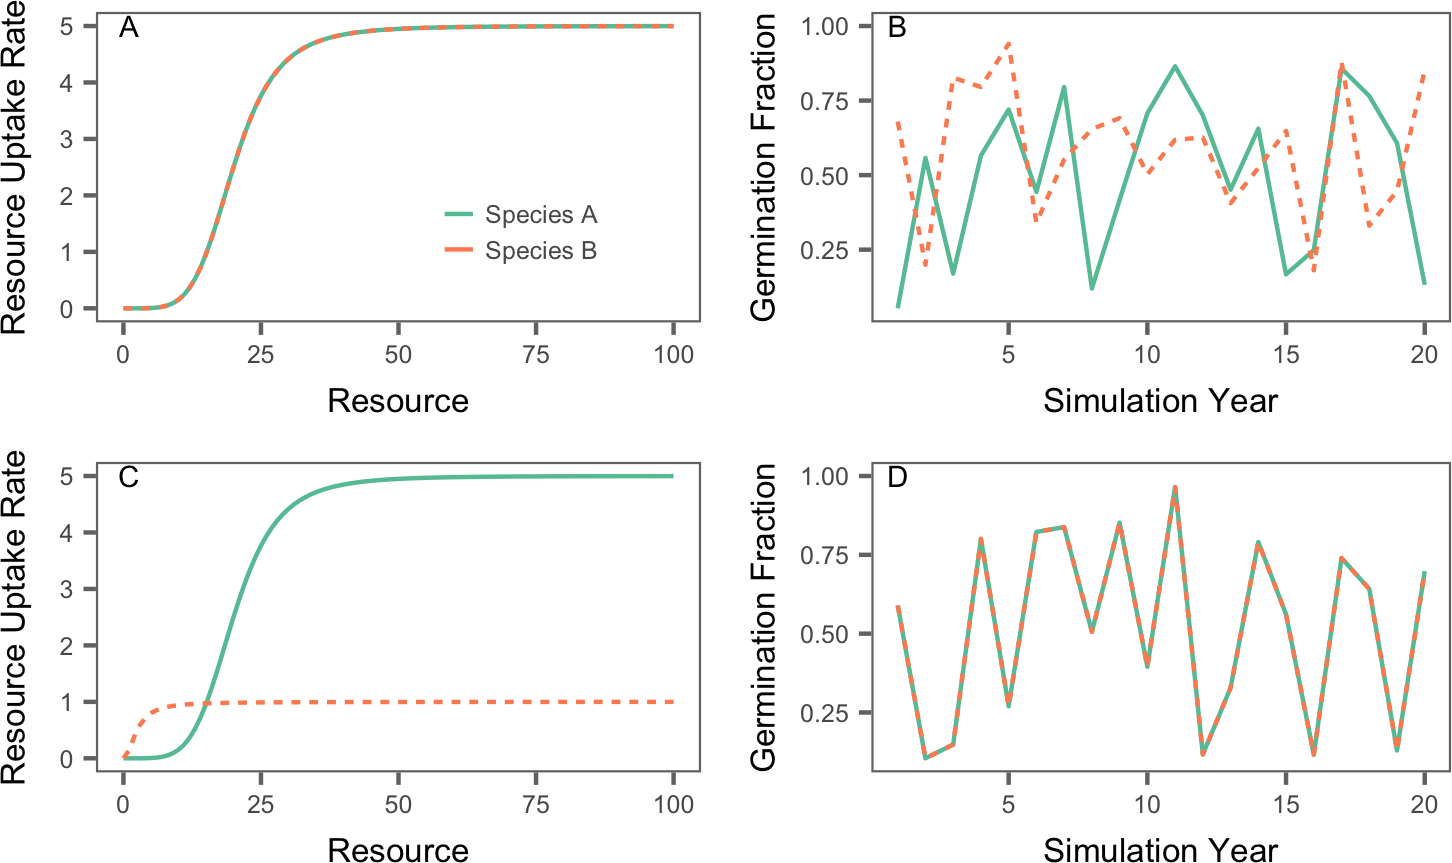
\includegraphics{components/figure/manuscript-model_types-1.png}
\caption{Resource uptake functions and example time series of
(un)correlated germination fractions for the storage effect (A,B) and
relative nonlinearity (C,D) formulations of the consumer-resource model.
The resource uptake functions for both species are equivalent for the
storage effect, but their dormant-to-live transition fractions
(\(\gamma\)) are uncorrelated in time. The opposite is true for relative
nonlinearity: the two species have unique resource uptake functions, but
their dormant-to-live transition fractions (\(\gamma\)) are perfectly
correlated in time.}
\end{figure}

\newpage{}

\begin{figure}[!ht]
  \centering
      \includegraphics[height=5in]{/Users/atredenn/Google_Drive/coexistence-stability_submission/figures/coex_stability_figure1.png}
  \caption{Variability of total community biomass as a function of species richness when coexistence is maintained by the storage effect (A,B) or relative nonlinearity (C,D). Top panels show results from simulations where environmental or resource variance determine the number species that coexist in a community. Bottom panels show results from simulations where environmental or resource variance is fixed at a level that allows coexistence of all four species, but species are removed to manipulate diversity. The left-hand panels represent regional diversity-variability relationships across natural diversity gradients, whereas the right-hand panels represent local diversity-variability relationships. Parameter values, where species are denoted by numeric subscripts: (A) $r_1 = r_2 = r_3 = r_4 = 0.2$, $a_1 = a_2 = a_3 = a_4 = 2$, $b_1 = b_2 = b_3 = b_4 = 2.5$, $\alpha_1 = 0.5, \alpha_2 = 0.49, \alpha_3 = 0.48, \alpha_4 = 0.47$, $\rho_1 = \rho_2 = \rho_3 = \rho_4 = 0$, $\sigma_E =$ variable; (B) $r_1 = r_2 = r_3 = r_4 = 0.2$, $a_1 = a_2 = a_3 = a_4 = 2$, $b_1 = b_2 = b_3 = b_4 = 2.5$, $\alpha_1 = 0.5, \alpha_2 = 0.49, \alpha_3 = 0.48, \alpha_4 = 0.47$, $\rho_1 = \rho_2 = \rho_3 = \rho_4 = -1/3$, $\sigma_E = 4$; (C) $r_1 = 0.2, r_2 = 1, r_3 = 2, r_4 = 5$, $a_1 = 2, a_2 = 5, a_3 = 10, a_4 = 25$, $b_1 = 2.5, b_2 = 20, b_3 = 30, b_4 = 45$, $\alpha_1 = \alpha_2 = \alpha_3 = \alpha_4 = 0.5$, $\rho_1 = \rho_2 = \rho_3 = \rho_4 = 1$, $\sigma(R^+) =$ variable; (D) $r_1 = 0.2, r_2 = 1, r_3 = 2, r_4 = 5$, $a_1 = 2, a_2 = 5, a_3 = 10, a_4 = 25$, $b_1 = 2.5, b_2 = 20, b_3 = 30, b_4 = 45$, $\alpha_1 = \alpha_2 = \alpha_3 = \alpha_4 = 0.5$, $\rho_1 = \rho_2 = \rho_3 = \rho_4 = 1$, $\sigma(R^+) =$ 1.2.}
\end{figure}

\newpage{}

\begin{figure}[!ht]
  \centering
      \includegraphics[height=5in]{/Users/atredenn/Google_Drive/coexistence-stability_submission/figures/coex_stability_figure2.png}
  \caption{The effect of increasing environmental variability on ecosystem variability when species coexist via the storage effect. Panels (A-C) show simulation results where species have slightly asymmetrical competitive effects, whereas panels (D-F) show results when competition is more asymmetric. Columns show results for different levels of correlations of species' environmental responses, $\rho$. Colored vertical lines show the magnitude of environmental variability at which each level of species richness first occurs. Parameter values are as in Figure 2A except for $\alpha$s: (A-C) $\alpha_1 = 0.5, \alpha_2 = 0.495, \alpha_3 = 0.49, \alpha_4 = 0.485$; (D-F) $\alpha_1 = 0.5, \alpha_2 = 0.49, \alpha_3 = 0.48, \alpha_4 = 0.47$.}
\end{figure}

\newpage{}

\begin{figure}[!ht]
  \centering
      \includegraphics[height=2.5in]{/Users/atredenn/Google_Drive/coexistence-stability_submission/figures/coex_stability_figure3.png}
  \caption{The effect of environmental variability on ecosystem variability when species coexist via relative nonlinearity. (A) The species pool increases from one to four species, with the fourth species being most unstable (e.g., resource conservative to resource acquisitive). Increasing environmental variability (the SD of annual resource availability) allows for greater species richness, but species additions do not modulate the effect of environmental variability on ecosystem variability. (B) The species pool increases from one to four species, with the fourth species being most stable (e.g., resource acquisitive to resrouce conservative). In this case, increasing environmental variability allows for greater realized species richness and can temper the effect of environmental variability. In (B), there is limited parameter space under which only three species coexist, which is why a three species community is missing. Parameter values are as in Figure 2C.}
\end{figure}

\newpage{}

\begin{figure}[!ht]
  \centering
      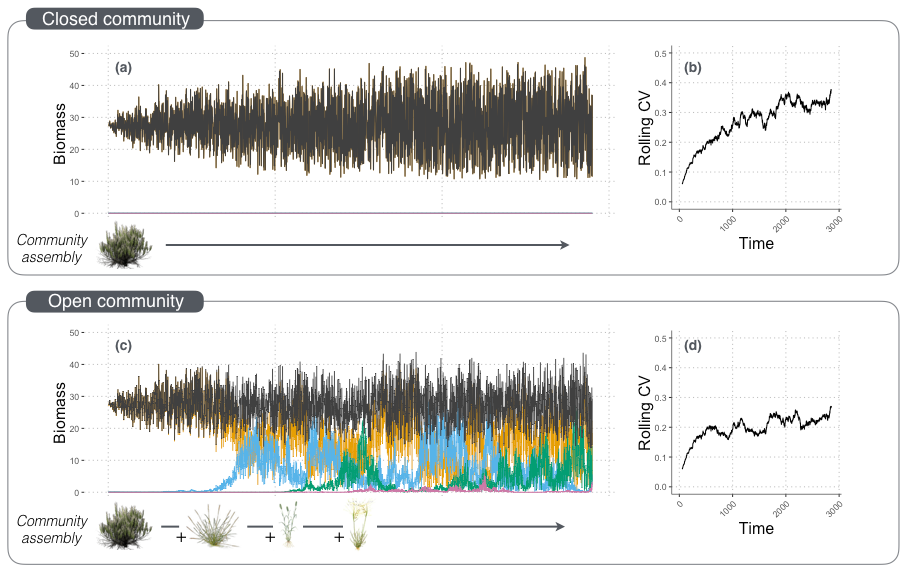
\includegraphics[height=4in]{./components/coexistence_stability_infographic_v2.png}
  \caption{Example of how species additions under increasing environmental variability can buffer ecosystem stability when species coexist via the storage effect. Environmental variability ($\sigma^2_E$) increases linearly with time on the \emph{x}-axis. (A) Time series of species' biomass (colored lines) in a closed community where colonization of new species is prevented and (B) its associated coefficient of variation (Rolling CV; calculated over 100-yr moving window) through time. (C) Time series of species' biomass in an open community where colonization by new species from the regional pool of four species becomes possible as environmental variation increases. The trajectory of total biomass CV in the open community (D) asymptotes at lower variability than in the closed community (B) due to the buffering effect of species richness. Parameter values are as in Figure 2A except for $\alpha$s: $\alpha_1 = 0.5, \alpha_2 = 0.494, \alpha_3 = 0.49, \alpha_4 = 0.483$.}
\end{figure}


\end{document}
